% !TeX program = pdflatex
\documentclass[russian,utf8,simple]{eskdtext}

% packages
%
% Тестовое наполнение текстом
% При написании работы - удалить пакет и комманды \lipsum
\usepackage{lipsum}
%
\usepackage{graphicx}
\usepackage{datetime}
\usepackage{enumitem} % for lists
\usepackage{ulem} % for underlining
\usepackage{lastpage} % Number of pages
\usepackage{hyperref} % Links in pdf

% setup
\newcommand{\FrontPageDepartment}{ИТ} %Факультет
\newcommand{\FrontPageSubdepartment}{САПР} %Кафедра
\newcommand{\WorkType}{Лабораторная работа №1} %Тип работы (заголовок)
\newcommand{\Subject}{Инструментальные средства разработки программного обеспечения} %по ... родительный падеж
\newcommand{\Topic}{Работа с системами контроля версий} %Тема
\newcommand{\Professor}{Пугин~Е.~В.} %Руководитель
\newcommand{\Student}{Гудкова~О.~Н.} %Студент
\newcommand{\Group}{ПКС-216} %Группа
\newcommand{\FrontPageDate}{\ddmmyyyydate\today} %Дата

\ESKDsignature{МИВУ 09.02.03} % Код специальности и тип работы

% eskdx setup
\ESKDletter{}{У}{}
\ESKDtitle{\WorkType

\Topic}
\ESKDchecker{\Professor}
\ESKDauthor{\Student}
\ESKDcolumnIX{МИ ВлГУ\\ \Group}

\addto\captionsrussian{\def\refname{Список использованных источников}}
\sloppy % split long lines

% graphics path
\graphicspath{{src/img/}}


% verbatim setup
\newcommand{\verbatimFont}{
\fontsize{10pt}{12pt}\selectfont
\baselineskip=1em
}


% workaround for regression in babel package on linux
\providecommand{\No}{\textnumero}


% remove vertical space from lists
%\renewcommand{\alph}[1]{\asbuk{#1}} % костыль для кирилической нумерации вместо латинской
\setlist{nolistsep} % убираем дополнительные вертикальные отступы вокруг списков
\setenumerate[1]{label=\arabic*), fullwidth, itemindent=\parindent,  listparindent=\parindent}
\setenumerate[2]{label=\arabic*), fullwidth, itemindent=\parindent, listparindent=\parindent, leftmargin=\parindent}
\setitemize{fullwidth, itemindent=\parindent, listparindent=\parindent}

% main document
\begin{document}
% Титул
\ESKDthisStyle{title}
\newlength{\frontpagefk} % Ширина поля Факультет/Кафедра
\setlength{\frontpagefk}{6cm}
\newlength{\frontpagerb} % Ширина надписей Руководитель/Студент и пр. под темой
\setlength{\frontpagerb}{6cm}
\newlength{\frontpagerbspace} % ??? (do not remove)
\setlength{\frontpagerbspace}{1cm}
\newlength{\FrontPageSubjSpace} % Ширина пробела до и после названия предмета
\setlength{\FrontPageSubjSpace}{1cm}
\newlength{\FrontPageTopicSpace} % Ширина пробела до и после темы
\setlength{\FrontPageTopicSpace}{0.5cm}

\thispagestyle{empty}
\begin{center}
{
\vspace*{-1.5cm}
\baselineskip=1.3em
{\small Министерство образования и науки Российской Федерации}\\
\textbf{Муромский институт (филиал)}\\
{\footnotesize федерального государственного бюджетного образовательного учреждения\\
высшего профессионального образования}\\
\textbf{<<Владимирский государственный университет\\
имени Александра Григорьевича и Николая Григорьевича\\
Столетовых>>\\
(МИВлГУ)\\}
}

\bigskip
\begin{tabular}{l c}
\textbf{Факультет}&\underline{\makebox[\frontpagefk]{\FrontPageDepartment}}\\
\textbf{Кафедра}&\underline{\makebox[\frontpagefk]{\FrontPageSubdepartment}}\\
\end{tabular}

\vspace{\fill}
\begin{Huge}
\textbf{\textsl{\WorkType}}
\end{Huge}

\vspace{\fill}
по \underline{\makebox[\FrontPageSubjSpace]{}\Subject\makebox[\FrontPageSubjSpace]{}}

\smallskip
\parbox{15cm}{\centering{Тема: \uline{\makebox[\FrontPageTopicSpace]{}\Topic\makebox[\FrontPageTopicSpace]{}}}}

\vspace{\fill}

\begin{flushright}
\makebox[\frontpagerb][c]{
\makebox[\frontpagerb][l]{Руководитель}\hspace{\frontpagerbspace}}

\smallskip
\makebox[\frontpagerb][c]{
\raisebox{-\baselineskip}{\shortstack{\underline{\makebox[\frontpagerb][l]{\Professor}}\\
\begin{footnotesize}
(фамилия, инициалы)
\end{footnotesize}}}\hspace{\frontpagerbspace}}

\bigskip
\makebox[\frontpagerb][c]{
\raisebox{-\baselineskip}{\shortstack{\underline{\makebox[\frontpagerb][l]{}}\\
\begin{footnotesize}
(подпись)\hfill(дата)
\end{footnotesize}}}\hspace{\frontpagerbspace}}

\newcommand{\frontpagerbstudent}[2]{ %
\makebox[\frontpagerb]{ %
\raisebox{-\baselineskip}{\shortstack{#1\ \underline{\makebox[\frontpagerb-\widthof{#1\ }][c]{#2}}\\
\begin{footnotesize}
\makebox[\widthof{#1\ }][c]{}\makebox[\frontpagerb-\widthof{#1\ }][c]{(группа)}
\end{footnotesize}}}\hspace{\frontpagerbspace}}
}

\bigskip
\makebox[\frontpagerb][c]{\frontpagerbstudent{Студент}{\Group}}

\smallskip
\makebox[\frontpagerb][c]{
\raisebox{-\baselineskip}{\shortstack{\underline{\makebox[\frontpagerb][l]{\Student}}\\
\begin{footnotesize}
(фамилия, инициалы)
\end{footnotesize}}}\hspace{\frontpagerbspace}}

\renewcommand{\dateseparator}{.}

\bigskip
\makebox[\frontpagerb][c]{
\raisebox{-\baselineskip}{\shortstack{\underline{\makebox[\frontpagerb][r]{\FrontPageDate}}\\
\begin{footnotesize}
(подпись)\hfill(дата)
\end{footnotesize}}}\hspace{\frontpagerbspace}}

\end{flushright}

\vspace{\fill}
Муром \the\year
\vspace*{-1cm}
\end{center}
\newpage



% Основной текст
\ESKDthisStyle{formII}
\begin{center}
Лабораторная работа №1.
\\
Тема: Работа с системами контроля версий.
\\
Цель: Изучить порядок клонирования репозитория на гитхабе и на компьютере.
 
\end{center}
Задание:
\begin{enumerate}
\item Зарегистрироваться на https://github.com/

\item Склонировать репозиторий шаблонов tex https://github.com/egorpugin/tex
 
\item Подготовить шаблон отчёта для лабораторных работ в LaTeX.

\item Загрузить шаблон в репозиторий tex.

\item Создать новый репозиторий для лабораторных работ на гитхабе.

\item Оформить отчёт и загрузить его в репозиторий для ЛР.
\end{enumerate}
Ход выполнения:
\\
Порядок клонирования репозитория на гитхабе.
\\
\begin{enumerate}
\item Нажать кнопку Fork (Клонировать)
\end{enumerate}

\begin{figure}[h]
\centering
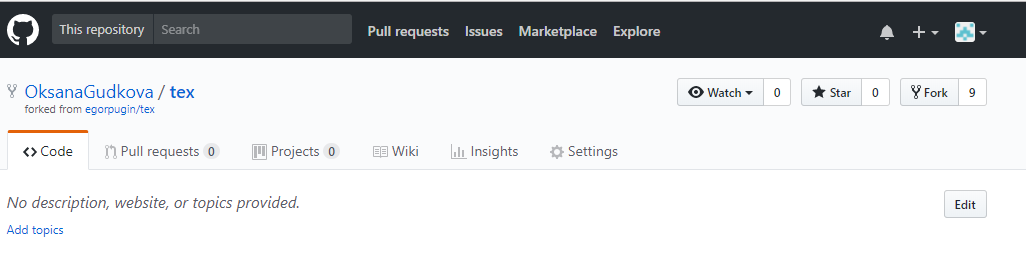
\includegraphics[scale=0.5]{s3}
\caption{Клонирования репозитория на гитхабе}
\label{fig:qwe}
\end{figure}
 
Порядок клонирования репозитория на компьютере.

\begin{figure}[h]
\centering
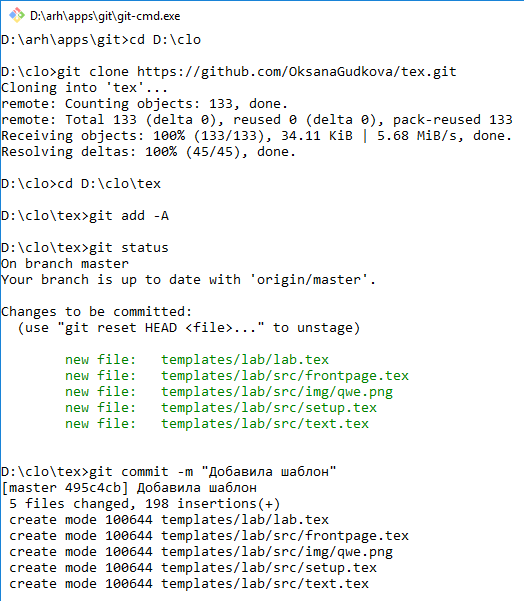
\includegraphics[scale=1]{s1}
\caption{Клонирования репозитория на компьютер, внесения новых файлов}
\label{fig:sk1}
\end{figure}

\begin{figure}[h]
\centering
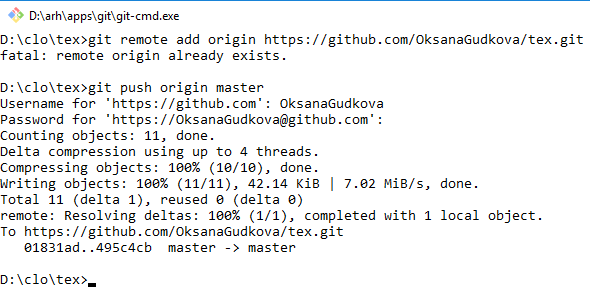
\includegraphics[scale=1]{s2}
\caption{Фиксация изменений и загрузка изменений на гитхаб}
\label{fig:sk2}
\end{figure}

\begin{figure}[h]
\centering
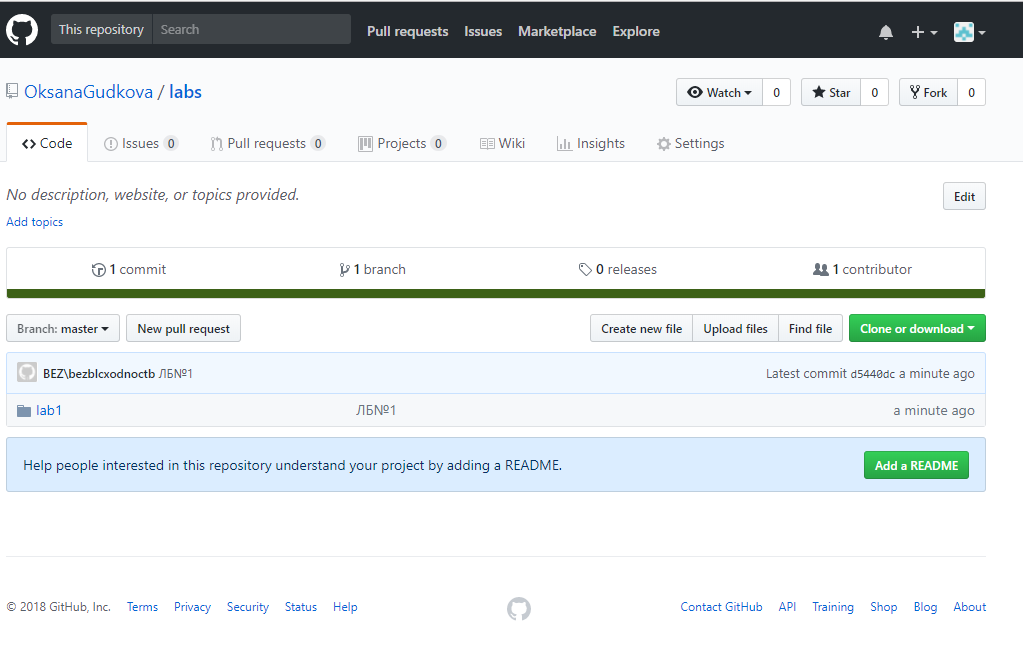
\includegraphics[scale=0.6]{s4}
\caption{Загрузка Лабораторной работы на гитхаб}
\label{fig:sk3}
Вывод: Изучила порядок клонирования репозитория на гитхабе и на компьютере.
\end{figure}




\newpage
\end{document}